% LaTeX rebuttal letter example. 
% 
% Copyright 2019 Friedemann Zenke, fzenke.net
%
% Based on examples by Dirk Eddelbuettel, Fran and others from 
% https://tex.stackexchange.com/questions/2317/latex-style-or-macro-for-detailed-response-to-referee-report
% 
% Licensed under cc by-sa 3.0 with attribution required.
% See https://creativecommons.org/licenses/by-sa/3.0/
% and https://stackoverflow.blog/2009/06/25/attribution-required/

\documentclass[11pt]{article}
\usepackage[utf8]{inputenc}
\usepackage{lipsum} % to generate some filler text
\usepackage{fullpage}

\usepackage{graphicx}
\usepackage{comment}
\usepackage{amsmath, amssymb}

%########################################################################################
%            						PACKAGES
%########################################################################################
\usepackage[pagebackref=true,bookmarks]{hyperref}
\hypersetup{
	unicode=false,
	pdftoolbar=true,
	pdfmenubar=true,
	pdffitwindow=false,     % window fit to page when opened
	pdfstartview={FitH},    % fits the width of the page to the window
	pdfkeywords={}, % list of keywords
	pdfnewwindow=true,      % links in new window
	colorlinks=true,       % false: boxed links; true: colored links
	linkcolor=red,          % color of internal links (change box color with linkbordercolor)
	citecolor=blue,        % color of links to bibliography
	filecolor=black,      % color of file links
	urlcolor=cyan           % color of external links
}
\usepackage{pdfpages}
%\usepackage{authblk} % for author affiliations
\usepackage{amsmath,amssymb,bbm,mathrsfs,mathtools,xfrac} %math stuff
\usepackage{amsthm}
%\newtheorem{theorem}{Theorem}
%\newtheorem{lemma}{Lemma}

%\usepackage{cleveref}
%\newcommand{\crefrangeconjunction}{--}
%\usepackage[nomarkers,figuresonly]{endfloat}

%\usepackage[sort]{natbib}   % bibliography omit 'round' option if you prefer square brackets
\usepackage{placeins} % for \FloatBarrier
\usepackage[utf8]{inputenc} % for french accents
\usepackage[T1]{fontenc} % for french accents
\usepackage{ctable} % load after tikz. used for tables
\usepackage{pifont}% http://ctan.org/pkg/pifont
\newcommand{\cmark}{\ding{51}}%
\newcommand{\xmark}{\ding{55}}%
\def\widebar#1{\overline{#1}}
\usepackage{array}
\newcolumntype{L}{>{\centering\arraybackslash}m{3cm}} % used for text wrapping in ctable
\usepackage{color, colortbl, xcolor, comment}
\usepackage{subfig}
%\usepackage{tcolorbox} % for box around text
%\usepackage[ruled,vlined,linesnumbered,noresetcount]{algorithm2e}
%\usepackage[ruled,vlined,noresetcount]{algorithm2e}
\usepackage{algorithm}
\usepackage{chngcntr} % for figure labels in appendix
%\usepackage[ruled,vlined,noresetcount]{algorithm2e}
\usepackage[noend]{algpseudocode}
\algrenewcommand\textproc{}% Used to be \textsc
\algdef{SE}[SUBALG]{Indent}{EndIndent}{}{\algorithmicend\ }%
\algtext*{Indent}
\algtext*{EndIndent}
%\usepackage[american]{babel}
%\let\tnote\relax

%\usepackage{csquotes}

\usepackage{pdflscape}
\usepackage{float} % for H in figures and tables
%\usepackage[style=apa,sortcites=true,sorting=nyt,backend=biber]{biblatex}
%\usepackage{epstopdf}

%\usepackage{tabulary}
%\usepackage{siunitx}
%\sisetup{output-exponent-marker=\ensuremath{\mathrm{e}}}
%\AtBeginEnvironment{tabulary}{\onehalfspacing}
%\usepackage{multirow}
%\usepackage{ctable} % NEED TO LOAD CTABLE AFTER TIKZ FOR SOME REASON
%\usepackage{array}
%\newcolumntype{L}{>{\centering\arraybackslash}m{3cm}} % used for text wrapping in ctable
%\usepackage{enumitem}
% These packages are all incorporated in the memoir class to one degree or another...


%%%Author macros
\def\tsc#1{\csdef{#1}{\textsc{\lowercase{#1}}\xspace}}
\tsc{WGM}
\tsc{QE}
\tsc{EP}
\tsc{PMS}
\tsc{BEC}
\tsc{DE}
%########################################################################################
%            						CUSTOM COMMANDS
%########################################################################################



\newcommand{\mb}[1]{\mathbf{#1}}
\newcommand{\bX}{\mathbf{\emph{X}}}
\newcommand{\bu}{\textbf{u}}
\newcommand{\bU}{\textbf{\emph{U}}}
\newcommand{\bV}{\textbf{\emph{V}}}
\newcommand{\bE}{\textbf{\emph{E}}}
\newcommand{\bb}{\textbf{\emph{b}}}
\newcommand{\bI}{\textbf{\emph{I}}}
\newcommand{\be}{\boldsymbol{\varepsilon}}
\newcommand{\bSigma}{\boldsymbol{\Sigma}}
\newcommand{\bLambda}{\boldsymbol{\Lambda}}
\newcommand{\bTheta}{\boldsymbol{\Theta}}
\newcommand{\balpha}{\boldsymbol{\alpha}}
\newcommand{\btau}{\boldsymbol{\tau}}
\newcommand{\bgamma}{\boldsymbol{\gamma}}
%\newcommand{\ltwonorm}[1]{\lVert #1 \rVert}
\newcommand{\mc}[2]{\multicolumn{#1}{c}{#2}}
\newcommand{\mcl}[2]{\multicolumn{#1}{l}{#2}}
\definecolor{Gray}{gray}{0.9}
\newcommand {\bs}{\boldsymbol}
%\newcommand{\norm}[1]{\left\Vert #1 \right\Vert}
\newcommand{\xf}{\mathcal{X}}
\newcommand{\pfrac}[2]{\left( \frac{#1}{#2}\right)}
\newcommand{\e}{{\mathsf E}}
\newcommand{\bt}{\boldsymbol{\theta}}
\newcommand{\bmu}{\boldsymbol{\mu}}
\newcommand{\bbeta}{\boldsymbol{\beta}}
\newcommand{\btheta}{\boldsymbol{\theta}}
\newcommand{\bPhi}{\boldsymbol{\Phi}}
\newcommand{\bPsi}{\boldsymbol{\Psi}}
\DeclareMathOperator*{\argmin}{arg\,min}
\DeclareMathOperator*{\argmax}{arg\,max}
\DeclareMathOperator{\diag}{diag} % operator and subscript

\DeclarePairedDelimiter\abs{\lvert}{\rvert}%
\DeclarePairedDelimiter\norm{\lVert}{\rVert}%

\global\long\def\ddd{,\ldots,}


\newcommand{\bthetastar}{\boldsymbol{\theta}^{*}}
\newcommand{\bThetastar}{\boldsymbol{\Theta}^{*}}
\newcommand{\bdelta}{\boldsymbol{\delta}}
\newcommand{\A}{\mathcal{A}}
\newcommand{\mH}{\mathcal{H}}
% import Eq and Section references from the main manuscript where needed
% \usepackage{xr}
% \externaldocument{manuscript}

% package needed for optional arguments
\usepackage{xifthen}
% define counters for reviewers and their points
\newcounter{reviewer}
\setcounter{reviewer}{0}
\newcounter{point}[reviewer]
\setcounter{point}{0}

% This refines the format of how the reviewer/point reference will appear.
\renewcommand{\thepoint}{P\,\thereviewer.\arabic{point}} 

% command declarations for reviewer points and our responses
\newcommand{\reviewersection}{\stepcounter{reviewer} \bigskip \hrule
                  \section*{Reviewer \thereviewer}}

\newenvironment{point}
   {\refstepcounter{point} \bigskip \noindent {\textbf{Reviewer~Point~\thepoint} } ---\ }
   {\par }

\newcommand{\shortpoint}[1]{\refstepcounter{point}  \bigskip \noindent 
	{\textbf{Reviewer~Point~\thepoint} } ---~#1\par }

\newenvironment{reply}
   {\medskip \noindent \begin{sf}\textbf{Reply}:\  }
   {\medskip \end{sf}}

\newcommand{\shortreply}[2][]{\medskip \noindent \begin{sf}\textbf{Reply}:\  #2
	\ifthenelse{\equal{#1}{}}{}{ \hfill \footnotesize (#1)}%
	\medskip \end{sf}}

\usepackage{natbib}

\begin{document}

\noindent\textbf{A Sparse Additive Model for High-Dimensional Interactions with an Exposure Variable} by Sahir R Bhatnagar, Tianyuan Lu, Amanda Lovato, David L Olds, Michael S Kobor, Michael J Meaney, Kieran O'Donnell, Yi Yang, Celia MT Greenwood.

\section*{Response to the reviewers}
% General intro text goes here
%We thank the reviewers for their critical assessment of our work. 
%In the following we address their concerns point by point. 

We thank the reviewers for their constructive comments, which we believe has significantly improved our manuscript. In this document, we reproduce the reviewers comments, and provide our response to each of them below. 

% Let's start point-by-point with Reviewer 1
\reviewersection

The paper proposes a method sail for detecting non-linear interactions with an environmental or exposure variable in high-dimensional settings where the strong or weak heredity constraints hold. The asymptotic properties are proved. To estimate unknown parameters, a computationally efficient algorithm with automatic tuning parameter selection is provided. In particular, an R package sail is made available on CRAN. Experiments conducted with simulations and real data validate the effectiveness of the proposed method.

In my opinion, the topic discussed in the paper is interesting and suitable to publish in CSDA. The organization and English quality of the paper is well-written. The theoretical and empirical studies seem to be convincing to show the effectiveness of the proposed method Sail. However, the following questions and comments may be useful for the authors to further improve the paper.



% Point one description 
\begin{point}
In the body part, the main steps of several algorithms are provided. However, the explanation and issues that should be paid attention to use these algorithms are not presented but postponed in appendix. I propose to add some descriptions of the algorithms in the body part.
\end{point}


\begin{reply}
Thank you for pointing this out. We have moved the more detailed description of the Algorithm from the appendix to the main text. 
\end{reply}

%%%%%%%%%%%%%%%%%%%%%%%%%%%%%%%%%%%%%%%%%%%%%%%%%%%%%%%%%%%%%%%%%%%%%%%%%%%%%%%%%%%%%%%%%%%%%%%%%%%
%%%%%%%%%%%%%%%%%%%%%%%%%%%%%%%%%%%%%%%%%%%%%%%%%%%%%%%%%%%%%%%%%%%%%%%%%%%%%%%%%%%%%%%%%%%%%%%%%%%
%%%%%%%%%%%%%%%%%%%%%%%%%%%%%%%%%%%%%%%%%%%%%%%%%%%%%%%%%%%%%%%%%%%%%%%%%%%%%%%%%%%%%%%%%%%%%%%%%%%%%%%
%%%%%%%%%%%%%%%%%%%%%%%%%%%%%%%%%%%%%%%%%%%%%%%%%%%%%%%%%%%%%%%%%%%%%%%%%%%%%%%%%%%%%%%%%%%%%%%%%%%
%%%%%%%%%%%%%%%%%%%%%%%%%%%%%%%%%%%%%%%%%%%%%%%%%%%%%%%%%%%%%%%%%%%%%%%%%%%%%%%%%%%%%%%%%%%%%%%%%%%
%%%%%%%%%%%%%%%%%%%%%%%%%%%%%%%%%%%%%%%%%%%%%%%%%%%%%%%%%%%%%%%%%%%%%%%%%%%%%%%%%%%%%%%%%%%%%%%%%%%%%%%
%%%%%%%%%%%%%%%%%%%%%%%%%%%%%%%%%%%%%%%%%%%%%%%%%%%%%%%%%%%%%%%%%%%%%%%%%%%%%%%%%%%%%%%%%%%%%%%%%%%
%%%%%%%%%%%%%%%%%%%%%%%%%%%%%%%%%%%%%%%%%%%%%%%%%%%%%%%%%%%%%%%%%%%%%%%%%%%%%%%%%%%%%%%%%%%%%%%%%%%
%%%%%%%%%%%%%%%%%%%%%%%%%%%%%%%%%%%%%%%%%%%%%%%%%%%%%%%%%%%%%%%%%%%%%%%%%%%%%%%%%%%%%%%%%%%%%%%%%%%%%%%


\begin{point}
The statements and symbols used in the paper are not very rigorous. For example, $Y_1, Y_2, \cdots, Y_n$ at the beginning of subsection 1.1 are in fact $n$ observations of the outcome variable. But the authors state $Y= (Y_1, Y_2, \cdots, Y_n)\in \mathbb{R}^n$ be a continuous outcome variable. The environmental variable $X_E$ has the similar problem.
\end{point}


\begin{reply}
Thank you for bringing this up. We have fixed this issue and changed the wording as follows:

\begin{quote}
    Let $Y \in \mathbb{R}$ be a continuous outcome variable, $E\in \mathbb{R}$ a binary or continous environment/exposure vector of known importance, and $X\in \mathbb{R}^p$ a vector of additional predictors, possibly high-dimensional. Assume that we have $n$ observations of each quantity denoted by $Y=(Y_1, \ldots, Y_n) \in \mathbb{R}^n$, \mbox{$X_E=(E_1, \ldots, E_n) \in \mathbb{R}^n$}, and \mbox{$\bX = (X_{1}^\top, \ldots, X_{p}^\top) \in \mathbb{R}^{n\times p}$}.
\end{quote}
\end{reply}


%%%%%%%%%%%%%%%%%%%%%%%%%%%%%%%%%%%%%%%%%%%%%%%%%%%%%%%%%%%%%%%%%%%%%%%%%%%%%%%%%%%%%%%%%%%%%%%%%%%
%%%%%%%%%%%%%%%%%%%%%%%%%%%%%%%%%%%%%%%%%%%%%%%%%%%%%%%%%%%%%%%%%%%%%%%%%%%%%%%%%%%%%%%%%%%%%%%%%%%
%%%%%%%%%%%%%%%%%%%%%%%%%%%%%%%%%%%%%%%%%%%%%%%%%%%%%%%%%%%%%%%%%%%%%%%%%%%%%%%%%%%%%%%%%%%%%%%%%%%%%%%
%%%%%%%%%%%%%%%%%%%%%%%%%%%%%%%%%%%%%%%%%%%%%%%%%%%%%%%%%%%%%%%%%%%%%%%%%%%%%%%%%%%%%%%%%%%%%%%%%%%
%%%%%%%%%%%%%%%%%%%%%%%%%%%%%%%%%%%%%%%%%%%%%%%%%%%%%%%%%%%%%%%%%%%%%%%%%%%%%%%%%%%%%%%%%%%%%%%%%%%
%%%%%%%%%%%%%%%%%%%%%%%%%%%%%%%%%%%%%%%%%%%%%%%%%%%%%%%%%%%%%%%%%%%%%%%%%%%%%%%%%%%%%%%%%%%%%%%%%%%%%%%
%%%%%%%%%%%%%%%%%%%%%%%%%%%%%%%%%%%%%%%%%%%%%%%%%%%%%%%%%%%%%%%%%%%%%%%%%%%%%%%%%%%%%%%%%%%%%%%%%%%
%%%%%%%%%%%%%%%%%%%%%%%%%%%%%%%%%%%%%%%%%%%%%%%%%%%%%%%%%%%%%%%%%%%%%%%%%%%%%%%%%%%%%%%%%%%%%%%%%%%
%%%%%%%%%%%%%%%%%%%%%%%%%%%%%%%%%%%%%%%%%%%%%%%%%%%%%%%%%%%%%%%%%%%%%%%%%%%%%%%%%%%%%%%%%%%%%%%%%%%%%%%


\begin{point}
In the paragraph under the formula (3), it was mentioned that $w_E$, $w_j$, $w_{JE}$ are non-negative penalty factors. I consider that this is not rigorous since they are actually some weight parameters to reflect the relative importance of each part in the penalty term. Here, lambda is the penalty factor that should be tuned by some technique. But the authors haven't explain the role of it in the paragraph. In addition, how can the parameters $w_E$, $w_j$, $w_{JE}$ be determined? Do they also be chosen based on cross-validation?
\end{point}


\begin{reply}
Thanks for this question. The penalty factors are what allow for the adaptive \texttt{sail} approach detailed in Section 2.3 which is similar to the adaptive lasso technique~\citep{zou2006adaptive}. More specifically, Algorithm 2 details how these parameters ($w_E$, $w_j$, $w_{JE}$) are determined. Briefly, this is done in three main steps: 
	\begin{enumerate}
		\item For a decreasing sequence $\lambda = \lambda_{max}, \ldots,\lambda_{min}$ and fixed $\alpha$ run the \sail ~algorithm and use cross-validation or a data splitting procedure to determine the optimal value for the tuning parameter: $\lambda^{[opt]} \in \left\lbrace \lambda_{max},\ldots, \lambda_{min} \right\rbrace$. Let $\widehat{\beta_E}^{[opt]}, \widehat{\btheta}_{j}^{[opt]}$ and $\widehat{\btau}_j^{[opt]}$ for $j=1, \ldots,p$ be the coefficient estimates corresponding to the model at $\lambda^{[opt]}$. Note that in this first step, the penalty factors ($w_E$, $w_j$, $w_{JE}$) are all set to be 1.
		\item Set the weights to be
		\begin{enumerate}
			\item[] $w_E = \left(\abs{\widehat{\beta_E}^{[opt]}}+1/n\right)^{-1}$, $w_j = \left(\Vert \widehat{\btheta}_{j}^{[opt]} \Vert_2 +1/n \right)^{-1}$,
			$w_{jE} = \left(\Vert\widehat{\btau_j}^{[opt]}\Vert_2 +1/n \right)^{-1}$ for $j=1, \ldots, p$
		\end{enumerate}
		The $1/n$ is added to avoid dividing by zero. 
		\item Run the \texttt{sail} ~algorithm again, but this time with the penalty factors defined in step 2), and use cross-validation or a data splitting procedure to choose the optimal value of $\lambda$.
	\end{enumerate}
	We have added some text in the paragraph under the formula (3) to point the reader to the adaptive \texttt{sail} algorithm for further details on how these weights are estimated.  
\end{reply}


%%%%%%%%%%%%%%%%%%%%%%%%%%%%%%%%%%%%%%%%%%%%%%%%%%%%%%%%%%%%%%%%%%%%%%%%%%%%%%%%%%%%%%%%%%%%%%%%%%%
%%%%%%%%%%%%%%%%%%%%%%%%%%%%%%%%%%%%%%%%%%%%%%%%%%%%%%%%%%%%%%%%%%%%%%%%%%%%%%%%%%%%%%%%%%%%%%%%%%%
%%%%%%%%%%%%%%%%%%%%%%%%%%%%%%%%%%%%%%%%%%%%%%%%%%%%%%%%%%%%%%%%%%%%%%%%%%%%%%%%%%%%%%%%%%%%%%%%%%%%%%%
%%%%%%%%%%%%%%%%%%%%%%%%%%%%%%%%%%%%%%%%%%%%%%%%%%%%%%%%%%%%%%%%%%%%%%%%%%%%%%%%%%%%%%%%%%%%%%%%%%%
%%%%%%%%%%%%%%%%%%%%%%%%%%%%%%%%%%%%%%%%%%%%%%%%%%%%%%%%%%%%%%%%%%%%%%%%%%%%%%%%%%%%%%%%%%%%%%%%%%%
%%%%%%%%%%%%%%%%%%%%%%%%%%%%%%%%%%%%%%%%%%%%%%%%%%%%%%%%%%%%%%%%%%%%%%%%%%%%%%%%%%%%%%%%%%%%%%%%%%%%%%%
%%%%%%%%%%%%%%%%%%%%%%%%%%%%%%%%%%%%%%%%%%%%%%%%%%%%%%%%%%%%%%%%%%%%%%%%%%%%%%%%%%%%%%%%%%%%%%%%%%%
%%%%%%%%%%%%%%%%%%%%%%%%%%%%%%%%%%%%%%%%%%%%%%%%%%%%%%%%%%%%%%%%%%%%%%%%%%%%%%%%%%%%%%%%%%%%%%%%%%%
%%%%%%%%%%%%%%%%%%%%%%%%%%%%%%%%%%%%%%%%%%%%%%%%%%%%%%%%%%%%%%%%%%%%%%%%%%%%%%%%%%%%%%%%%%%%%%%%%%%%%%%


\begin{point}
On page 14, it is mentioned that the environment variable is centralized and then the method sail is applied. I wonder why the environmental variable also needed to be centralized. If it is a binary variable, should it be also centralized?
\end{point}


\begin{reply}
Thanks for pointing this out. Since we place no restriction on $X_E$ (i.e. it can be binary or continuous), we always center it. We agree that binary variables need not be centralized and this will not have an impact on the estimates for $\beta_E$. We centered the binary environment variable because our computational algorithm assumes that all variables have been centered by their mean, irrespective of the variable type. This centering will subsequently affect the estimate of the intercept. We have added the text below to the computation Section 2 to clarify why we center all variables prior to fitting the \texttt{sail} method:
\begin{quote}
    We assume that $Y$, $\bPsi_j$, $X_E$ and $X_E \circ \bPsi_j$ have been centered by their sample means $\widebar{Y}$, $\widebar{\bPsi}_j$, $\widebar{X}_E$, and $\widebar{X_E \circ \bPsi_j}$, respectively. Here, $\widebar{\bPsi}_j \in \mathbb{R}^{m_j}$ and $\widebar{X_E \circ \bPsi_j}\in \mathbb{R}^{m_j}$  represent the column means of $\bPsi_j$ and $X_E \circ \bPsi_j$, respectively. Since the intercept ($\beta_0$) is not penalized and all variables have been centered, we can omit it from the loss function and compute it once the algorithm has converged for all other parameters.
\end{quote}

\end{reply}


%%%%%%%%%%%%%%%%%%%%%%%%%%%%%%%%%%%%%%%%%%%%%%%%%%%%%%%%%%%%%%%%%%%%%%%%%%%%%%%%%%%%%%%%%%%%%%%%%%%
%%%%%%%%%%%%%%%%%%%%%%%%%%%%%%%%%%%%%%%%%%%%%%%%%%%%%%%%%%%%%%%%%%%%%%%%%%%%%%%%%%%%%%%%%%%%%%%%%%%
%%%%%%%%%%%%%%%%%%%%%%%%%%%%%%%%%%%%%%%%%%%%%%%%%%%%%%%%%%%%%%%%%%%%%%%%%%%%%%%%%%%%%%%%%%%%%%%%%%%%%%%
%%%%%%%%%%%%%%%%%%%%%%%%%%%%%%%%%%%%%%%%%%%%%%%%%%%%%%%%%%%%%%%%%%%%%%%%%%%%%%%%%%%%%%%%%%%%%%%%%%%
%%%%%%%%%%%%%%%%%%%%%%%%%%%%%%%%%%%%%%%%%%%%%%%%%%%%%%%%%%%%%%%%%%%%%%%%%%%%%%%%%%%%%%%%%%%%%%%%%%%
%%%%%%%%%%%%%%%%%%%%%%%%%%%%%%%%%%%%%%%%%%%%%%%%%%%%%%%%%%%%%%%%%%%%%%%%%%%%%%%%%%%%%%%%%%%%%%%%%%%%%%%
%%%%%%%%%%%%%%%%%%%%%%%%%%%%%%%%%%%%%%%%%%%%%%%%%%%%%%%%%%%%%%%%%%%%%%%%%%%%%%%%%%%%%%%%%%%%%%%%%%%
%%%%%%%%%%%%%%%%%%%%%%%%%%%%%%%%%%%%%%%%%%%%%%%%%%%%%%%%%%%%%%%%%%%%%%%%%%%%%%%%%%%%%%%%%%%%%%%%%%%
%%%%%%%%%%%%%%%%%%%%%%%%%%%%%%%%%%%%%%%%%%%%%%%%%%%%%%%%%%%%%%%%%%%%%%%%%%%%%%%%%%%%%%%%%%%%%%%%%%%%%%%


\begin{point}
In the last paragraph of section 3, it is mentioned that $\phi_m^{init}$ is an initial sqrt(n)-consistent estimate of $\phi*_m$. I wonder how we can obtain this type of $\phi_m^{init}$ in practice. Does this estimate have large influence on the performance of the whole method?
\end{point}


\begin{reply}
Thanks for this question. This is directly related to the comment about the penalty factors ($w_E$, $w_j$, $w_{JE}$). In practice, we use the \texttt{sail} algorithm to obtain the $\phi_m^{init}$ as described in Algorithm 2 in the main paper (we also restate the algorithm in our response to comment 1.3 above). In Lemma 1 and Theorem 1, we prove the existence of a local minimizer of our objective function, and that the \texttt{sail} estimator is indeed $\sqrt{n}$-consistent. 
\end{reply}


%%%%%%%%%%%%%%%%%%%%%%%%%%%%%%%%%%%%%%%%%%%%%%%%%%%%%%%%%%%%%%%%%%%%%%%%%%%%%%%%%%%%%%%%%%%%%%%%%%%
%%%%%%%%%%%%%%%%%%%%%%%%%%%%%%%%%%%%%%%%%%%%%%%%%%%%%%%%%%%%%%%%%%%%%%%%%%%%%%%%%%%%%%%%%%%%%%%%%%%
%%%%%%%%%%%%%%%%%%%%%%%%%%%%%%%%%%%%%%%%%%%%%%%%%%%%%%%%%%%%%%%%%%%%%%%%%%%%%%%%%%%%%%%%%%%%%%%%%%%%%%%
%%%%%%%%%%%%%%%%%%%%%%%%%%%%%%%%%%%%%%%%%%%%%%%%%%%%%%%%%%%%%%%%%%%%%%%%%%%%%%%%%%%%%%%%%%%%%%%%%%%
%%%%%%%%%%%%%%%%%%%%%%%%%%%%%%%%%%%%%%%%%%%%%%%%%%%%%%%%%%%%%%%%%%%%%%%%%%%%%%%%%%%%%%%%%%%%%%%%%%%
%%%%%%%%%%%%%%%%%%%%%%%%%%%%%%%%%%%%%%%%%%%%%%%%%%%%%%%%%%%%%%%%%%%%%%%%%%%%%%%%%%%%%%%%%%%%%%%%%%%%%%%
%%%%%%%%%%%%%%%%%%%%%%%%%%%%%%%%%%%%%%%%%%%%%%%%%%%%%%%%%%%%%%%%%%%%%%%%%%%%%%%%%%%%%%%%%%%%%%%%%%%
%%%%%%%%%%%%%%%%%%%%%%%%%%%%%%%%%%%%%%%%%%%%%%%%%%%%%%%%%%%%%%%%%%%%%%%%%%%%%%%%%%%%%%%%%%%%%%%%%%%
%%%%%%%%%%%%%%%%%%%%%%%%%%%%%%%%%%%%%%%%%%%%%%%%%%%%%%%%%%%%%%%%%%%%%%%%%%%%%%%%%%%%%%%%%%%%%%%%%%%%%%%


\begin{point}
In simulations and real-data experiments, it is mentioned that the tuning parameters are selected by 10-fold cross-validation. I wonder what type of metric is used in cross-validation in each situation. In section 5.2, AUC is used to determine the optimal tuning parameters. But in simulations and subsection 5.1, I guessed that prediction accuracy is utilized according to the contexts. Why different metrics are used in different situations? Does it have some special reasons and benefits to do in this manner?
\end{point}


\begin{reply}
We agree that there are many choices of selecting the optimal tuning parameter. In the simulation studies, we used a sample splitting approach (last paragraph of Section 4.2), where the training set was used to fit the model and the validation set was used to select the optimal tuning parameter corresponding to the minimum prediction mean squared error (MSE). This is a common technique in simulation studies since we have the luxury of creating as much data as we want. This has two benefits: 1) it reduces computational cost since we only have to fit the model once for a sequence of tuning parameters and 2) we obtain an unbiased estimate of the prediction error (see for example~\citet{hastie2020best,haris2016convex}). This is also the approach we took in the second real data analysis (Section 5.2) because we had enough observations ($n= 8,873$). In the first real-data analysis (Section 5.1), we use cross-validation because we don't have enough data for the sample splitting approach ($n=189$). For the metric used to select the tuning parameter, we follow~\citet{friedman2010regularization}, who use the mean squared prediction error for continuous responses and the AUC for binary responses. 
\end{reply}


%%%%%%%%%%%%%%%%%%%%%%%%%%%%%%%%%%%%%%%%%%%%%%%%%%%%%%%%%%%%%%%%%%%%%%%%%%%%%%%%%%%%%%%%%%%%%%%%%%%
%%%%%%%%%%%%%%%%%%%%%%%%%%%%%%%%%%%%%%%%%%%%%%%%%%%%%%%%%%%%%%%%%%%%%%%%%%%%%%%%%%%%%%%%%%%%%%%%%%%
%%%%%%%%%%%%%%%%%%%%%%%%%%%%%%%%%%%%%%%%%%%%%%%%%%%%%%%%%%%%%%%%%%%%%%%%%%%%%%%%%%%%%%%%%%%%%%%%%%%%%%%
%%%%%%%%%%%%%%%%%%%%%%%%%%%%%%%%%%%%%%%%%%%%%%%%%%%%%%%%%%%%%%%%%%%%%%%%%%%%%%%%%%%%%%%%%%%%%%%%%%%
%%%%%%%%%%%%%%%%%%%%%%%%%%%%%%%%%%%%%%%%%%%%%%%%%%%%%%%%%%%%%%%%%%%%%%%%%%%%%%%%%%%%%%%%%%%%%%%%%%%
%%%%%%%%%%%%%%%%%%%%%%%%%%%%%%%%%%%%%%%%%%%%%%%%%%%%%%%%%%%%%%%%%%%%%%%%%%%%%%%%%%%%%%%%%%%%%%%%%%%%%%%
%%%%%%%%%%%%%%%%%%%%%%%%%%%%%%%%%%%%%%%%%%%%%%%%%%%%%%%%%%%%%%%%%%%%%%%%%%%%%%%%%%%%%%%%%%%%%%%%%%%
%%%%%%%%%%%%%%%%%%%%%%%%%%%%%%%%%%%%%%%%%%%%%%%%%%%%%%%%%%%%%%%%%%%%%%%%%%%%%%%%%%%%%%%%%%%%%%%%%%%
%%%%%%%%%%%%%%%%%%%%%%%%%%%%%%%%%%%%%%%%%%%%%%%%%%%%%%%%%%%%%%%%%%%%%%%%%%%%%%%%%%%%%%%%%%%%%%%%%%%%%%%


\begin{point}
In subsection 4.1, I wonder how lasso and adaptive lasso is applied to other situations, like linear interactions and non-linear main effects. Should we consider all interactions between each pair of covariates plus the original covariates as the input variables of lasso or adaptive lasso?
\end{point}


\begin{reply}
Thanks for this question. The model you are describing is sometimes referred to in the literature as the \textit{all-pairs} lasso~\citep{bien2013lasso}. The input design matrix is indeed the main effects along with all the interactions $[X_1, X_2, \ldots, X_p, X_E, X_1:X_E, X_2:X_E, \ldots, X_p:X_E]$. In Section 1.1 we state that the issue with this approach is that since no constraint is placed on the structure of the model, it is possible that an estimated interaction term is non-zero while the corresponding main effects are zero. The same principle could be applied to non-linear effects. That is, we could use the input design matrix $[f(X_1), f(X_2), \ldots, f(X_p), X_E, f(X_1):X_E, f(X_2):X_E, \ldots, f(X_p):X_E]$, where $f(\cdot)$ is a non-linear transformation of the main effects. The same issue arises however, in that the heredity property is violated. We did not explore this option in our simulations because the lasso was not intended for this purpose. We instead focused on specialized approaches intended for interaction selection while satisfying the heredity property.  
\end{reply}


%%%%%%%%%%%%%%%%%%%%%%%%%%%%%%%%%%%%%%%%%%%%%%%%%%%%%%%%%%%%%%%%%%%%%%%%%%%%%%%%%%%%%%%%%%%%%%%%%%%
%%%%%%%%%%%%%%%%%%%%%%%%%%%%%%%%%%%%%%%%%%%%%%%%%%%%%%%%%%%%%%%%%%%%%%%%%%%%%%%%%%%%%%%%%%%%%%%%%%%
%%%%%%%%%%%%%%%%%%%%%%%%%%%%%%%%%%%%%%%%%%%%%%%%%%%%%%%%%%%%%%%%%%%%%%%%%%%%%%%%%%%%%%%%%%%%%%%%%%%%%%%
%%%%%%%%%%%%%%%%%%%%%%%%%%%%%%%%%%%%%%%%%%%%%%%%%%%%%%%%%%%%%%%%%%%%%%%%%%%%%%%%%%%%%%%%%%%%%%%%%%%
%%%%%%%%%%%%%%%%%%%%%%%%%%%%%%%%%%%%%%%%%%%%%%%%%%%%%%%%%%%%%%%%%%%%%%%%%%%%%%%%%%%%%%%%%%%%%%%%%%%
%%%%%%%%%%%%%%%%%%%%%%%%%%%%%%%%%%%%%%%%%%%%%%%%%%%%%%%%%%%%%%%%%%%%%%%%%%%%%%%%%%%%%%%%%%%%%%%%%%%%%%%
%%%%%%%%%%%%%%%%%%%%%%%%%%%%%%%%%%%%%%%%%%%%%%%%%%%%%%%%%%%%%%%%%%%%%%%%%%%%%%%%%%%%%%%%%%%%%%%%%%%
%%%%%%%%%%%%%%%%%%%%%%%%%%%%%%%%%%%%%%%%%%%%%%%%%%%%%%%%%%%%%%%%%%%%%%%%%%%%%%%%%%%%%%%%%%%%%%%%%%%
%%%%%%%%%%%%%%%%%%%%%%%%%%%%%%%%%%%%%%%%%%%%%%%%%%%%%%%%%%%%%%%%%%%%%%%%%%%%%%%%%%%%%%%%%%%%%%%%%%%%%%%


\begin{point}
Please the authors to check the information of each reference to make sure that the provided information is complete and correct. I doubt that the page numbers of Ning et al.(2018), Zou and Zhang(2019) are incorrect.
\end{point}


\begin{reply}
Thanks for pointing this out. We have fixed the references. 
\end{reply}

%%%%%%%%%%%%%%%%%%%%%%%%%%%%%%%%%%%%%%%%%%%%%%%%%%%%%%%%%%%%%%%%%%%%%%%%%%%%%%%%%%%%%%%%%%%%%%%%%%%
%%%%%%%%%%%%%%%%%%%%%%%%%%%%%%%%%%%%%%%%%%%%%%%%%%%%%%%%%%%%%%%%%%%%%%%%%%%%%%%%%%%%%%%%%%%%%%%%%%%
%%%%%%%%%%%%%%%%%%%%%%%%%%%%%%%%%%%%%%%%%%%%%%%%%%%%%%%%%%%%%%%%%%%%%%%%%%%%%%%%%%%%%%%%%%%%%%%%%%%%%%%
%%%%%%%%%%%%%%%%%%%%%%%%%%%%%%%%%%%%%%%%%%%%%%%%%%%%%%%%%%%%%%%%%%%%%%%%%%%%%%%%%%%%%%%%%%%%%%%%%%%
%%%%%%%%%%%%%%%%%%%%%%%%%%%%%%%%%%%%%%%%%%%%%%%%%%%%%%%%%%%%%%%%%%%%%%%%%%%%%%%%%%%%%%%%%%%%%%%%%%%
%%%%%%%%%%%%%%%%%%%%%%%%%%%%%%%%%%%%%%%%%%%%%%%%%%%%%%%%%%%%%%%%%%%%%%%%%%%%%%%%%%%%%%%%%%%%%%%%%%%%%%%
%%%%%%%%%%%%%%%%%%%%%%%%%%%%%%%%%%%%%%%%%%%%%%%%%%%%%%%%%%%%%%%%%%%%%%%%%%%%%%%%%%%%%%%%%%%%%%%%%%%
%%%%%%%%%%%%%%%%%%%%%%%%%%%%%%%%%%%%%%%%%%%%%%%%%%%%%%%%%%%%%%%%%%%%%%%%%%%%%%%%%%%%%%%%%%%%%%%%%%%
%%%%%%%%%%%%%%%%%%%%%%%%%%%%%%%%%%%%%%%%%%%%%%%%%%%%%%%%%%%%%%%%%%%%%%%%%%%%%%%%%%%%%%%%%%%%%%%%%%%%%%%

%\section*{Reviewer 2} %remove after done

\reviewersection

In this paper, the authors introduced a sparse version of allowing a model with non-linear interactions. Primarily, only one key exposure variable is allowed in the proposed model.  From the numerical study, when the true model follows the ``strong heredity principle", the performance is best.


\begin{point}
I think that the introduction seems to be too long.
\end{point}


\begin{reply}
Thanks for pointing this out. We have removed an entire paragraph from the introduction. We found it difficult to remove more, without significantly affecting the flow of the paper. 
\end{reply}




%%%%%%%%%%%%%%%%%%%%%%%%%%%%%%%%%%%%%%%%%%%%%%%%%%%%%%%%%%%%%%%%%%%%%%%%%%%%%%%%%%%%%%%%%%%%%%%%%%%
%%%%%%%%%%%%%%%%%%%%%%%%%%%%%%%%%%%%%%%%%%%%%%%%%%%%%%%%%%%%%%%%%%%%%%%%%%%%%%%%%%%%%%%%%%%%%%%%%%%
%%%%%%%%%%%%%%%%%%%%%%%%%%%%%%%%%%%%%%%%%%%%%%%%%%%%%%%%%%%%%%%%%%%%%%%%%%%%%%%%%%%%%%%%%%%%%%%%%%%%%%%
%%%%%%%%%%%%%%%%%%%%%%%%%%%%%%%%%%%%%%%%%%%%%%%%%%%%%%%%%%%%%%%%%%%%%%%%%%%%%%%%%%%%%%%%%%%%%%%%%%%
%%%%%%%%%%%%%%%%%%%%%%%%%%%%%%%%%%%%%%%%%%%%%%%%%%%%%%%%%%%%%%%%%%%%%%%%%%%%%%%%%%%%%%%%%%%%%%%%%%%
%%%%%%%%%%%%%%%%%%%%%%%%%%%%%%%%%%%%%%%%%%%%%%%%%%%%%%%%%%%%%%%%%%%%%%%%%%%%%%%%%%%%%%%%%%%%%%%%%%%%%%%
%%%%%%%%%%%%%%%%%%%%%%%%%%%%%%%%%%%%%%%%%%%%%%%%%%%%%%%%%%%%%%%%%%%%%%%%%%%%%%%%%%%%%%%%%%%%%%%%%%%
%%%%%%%%%%%%%%%%%%%%%%%%%%%%%%%%%%%%%%%%%%%%%%%%%%%%%%%%%%%%%%%%%%%%%%%%%%%%%%%%%%%%%%%%%%%%%%%%%%%
%%%%%%%%%%%%%%%%%%%%%%%%%%%%%%%%%%%%%%%%%%%%%%%%%%%%%%%%%%%%%%%%%%%%%%%%%%%%%%%%%%%%%%%%%%%%%%%%%%%%%%%


\begin{point}
The notation of sections 1, 2 is not consistent. For example, in section 2.2(weak heredity), the reparametrization $\alpha_j$ should be $\tau_j$ because equation (2) has no $\alpha_j$ terms.
Also, Equations (4) and (6) have similar parameterization repeatedly. A summarized table about models, reparametrization, penalty terms helps understand the proposed method under strong/weak heredity principles.
\end{point}


\begin{reply}
Thank you for pointing out this issue. We have fixed the error. We have also added a summary table in the main text which shows the model types, reparametrization and penalty as follows:

\begin{table}[H]
	\centering
		\caption{Summary of reparametrization and penalty terms for strong and weak heredity \texttt{sail} model. Note that the penalty terms are identical for both model types, i.e., the reparametrization only affects the likelihood term of the objective function. }
		\label{tab:reparam}
		\begin{tabular}{lll}
			\hline
	Model      &  Reparametrization & Penalty\\
	\hline
\multicolumn{1}{m{3cm}}{Strong heredity}    &    $\btau_{j} = \gamma_{jE} \beta_E \btheta_j $  & \multicolumn{1}{m{8cm}}{$\lambda (1-\alpha)  \left( w_E \abs{\beta_E} + \sum_{j=1}^{p} w_j \norm{\btheta_j}_2 \right) +  \lambda\alpha \sum_{j=1}^{p} w_{jE} \abs{\gamma_{jE}}$}         \\
\multicolumn{1}{m{3cm}}{Weak heredity} &    $\btau_{j} = \gamma_{jE}(\beta_E \cdot \mb{1}_{m_j} +  \btheta_j)$   & \multicolumn{1}{m{8cm}}{$\lambda (1-\alpha)  \left( w_E \abs{\beta_E} + \sum_{j=1}^{p} w_j \norm{\btheta_j}_2 \right) +  \lambda\alpha \sum_{j=1}^{p} w_{jE} \abs{\gamma_{jE}}$} \\
			\hline
		\end{tabular}
\end{table}
\end{reply}


%%%%%%%%%%%%%%%%%%%%%%%%%%%%%%%%%%%%%%%%%%%%%%%%%%%%%%%%%%%%%%%%%%%%%%%%%%%%%%%%%%%%%%%%%%%%%%%%%%%
%%%%%%%%%%%%%%%%%%%%%%%%%%%%%%%%%%%%%%%%%%%%%%%%%%%%%%%%%%%%%%%%%%%%%%%%%%%%%%%%%%%%%%%%%%%%%%%%%%%
%%%%%%%%%%%%%%%%%%%%%%%%%%%%%%%%%%%%%%%%%%%%%%%%%%%%%%%%%%%%%%%%%%%%%%%%%%%%%%%%%%%%%%%%%%%%%%%%%%%%%%%
%%%%%%%%%%%%%%%%%%%%%%%%%%%%%%%%%%%%%%%%%%%%%%%%%%%%%%%%%%%%%%%%%%%%%%%%%%%%%%%%%%%%%%%%%%%%%%%%%%%
%%%%%%%%%%%%%%%%%%%%%%%%%%%%%%%%%%%%%%%%%%%%%%%%%%%%%%%%%%%%%%%%%%%%%%%%%%%%%%%%%%%%%%%%%%%%%%%%%%%
%%%%%%%%%%%%%%%%%%%%%%%%%%%%%%%%%%%%%%%%%%%%%%%%%%%%%%%%%%%%%%%%%%%%%%%%%%%%%%%%%%%%%%%%%%%%%%%%%%%%%%%
%%%%%%%%%%%%%%%%%%%%%%%%%%%%%%%%%%%%%%%%%%%%%%%%%%%%%%%%%%%%%%%%%%%%%%%%%%%%%%%%%%%%%%%%%%%%%%%%%%%
%%%%%%%%%%%%%%%%%%%%%%%%%%%%%%%%%%%%%%%%%%%%%%%%%%%%%%%%%%%%%%%%%%%%%%%%%%%%%%%%%%%%%%%%%%%%%%%%%%%
%%%%%%%%%%%%%%%%%%%%%%%%%%%%%%%%%%%%%%%%%%%%%%%%%%%%%%%%%%%%%%%%%%%%%%%%%%%%%%%%%%%%%%%%%%%%%%%%%%%%%%%


\begin{point}
In measuring the variable section's ability, selections of other variables are affected significantly by the selection of $X_E$. How to evaluate the effect of $X_E$ in TPR? For example, "TPR" of $X_E$ only. Small simulations or some discussions are necessary.
\end{point}


\begin{reply}
We agree with this assessment. The premise of our method is built upon the fact that there is an exposure/environment variable with known importance. As such, all of our data generating mechanisms include an important exposure effect. We have evaluated the variable selection rates of the strong heredity \texttt{sail} method and reported the results in a figure shown in Supplemental Section C (Figure 8). We have also added a discussion of these results in the simulation section results (Section 4.3). Figure~\ref{fig:upset} is one example of the figure we have included in the supplemental section. It represents the model selection results across all simulation replications for scenario 1a). For example, we see that the set of variables $\left\lbrace X1, X3, X4, E, X3:E, X4:E \right\rbrace$ was selected in 131 of the replications. We can see that the environment variable is always selected across all replications.  

\begin{figure}[h]
    \centering

\includegraphics[width=\textwidth]{figure/upset_selection_sail_paramIndex1.pdf}
    \caption{Model selection results for strong heredity \texttt{sail} method. Shown are the selected models and their frequencies. We can see that the environment variable is always selected across all simulation scenarios and replications.}
    \label{fig:upset}
\end{figure}
\end{reply}

\FloatBarrier
%%%%%%%%%%%%%%%%%%%%%%%%%%%%%%%%%%%%%%%%%%%%%%%%%%%%%%%%%%%%%%%%%%%%%%%%%%%%%%%%%%%%%%%%%%%%%%%%%%%
%%%%%%%%%%%%%%%%%%%%%%%%%%%%%%%%%%%%%%%%%%%%%%%%%%%%%%%%%%%%%%%%%%%%%%%%%%%%%%%%%%%%%%%%%%%%%%%%%%%
%%%%%%%%%%%%%%%%%%%%%%%%%%%%%%%%%%%%%%%%%%%%%%%%%%%%%%%%%%%%%%%%%%%%%%%%%%%%%%%%%%%%%%%%%%%%%%%%%%%%%%%
%%%%%%%%%%%%%%%%%%%%%%%%%%%%%%%%%%%%%%%%%%%%%%%%%%%%%%%%%%%%%%%%%%%%%%%%%%%%%%%%%%%%%%%%%%%%%%%%%%%
%%%%%%%%%%%%%%%%%%%%%%%%%%%%%%%%%%%%%%%%%%%%%%%%%%%%%%%%%%%%%%%%%%%%%%%%%%%%%%%%%%%%%%%%%%%%%%%%%%%
%%%%%%%%%%%%%%%%%%%%%%%%%%%%%%%%%%%%%%%%%%%%%%%%%%%%%%%%%%%%%%%%%%%%%%%%%%%%%%%%%%%%%%%%%%%%%%%%%%%%%%%
%%%%%%%%%%%%%%%%%%%%%%%%%%%%%%%%%%%%%%%%%%%%%%%%%%%%%%%%%%%%%%%%%%%%%%%%%%%%%%%%%%%%%%%%%%%%%%%%%%%
%%%%%%%%%%%%%%%%%%%%%%%%%%%%%%%%%%%%%%%%%%%%%%%%%%%%%%%%%%%%%%%%%%%%%%%%%%%%%%%%%%%%%%%%%%%%%%%%%%%
%%%%%%%%%%%%%%%%%%%%%%%%%%%%%%%%%%%%%%%%%%%%%%%%%%%%%%%%%%%%%%%%%%%%%%%%%%%%%%%%%%%%%%%%%%%%%%%%%%%%%%%


\begin{point}
Is only the linear effect of the main exposure variable $X_E$ allowed? Otherwise, the simulation can include the non-linear effect of $X_E$.
\end{point}


\begin{reply}
This is indeed a limitation of our current approach. We mentioned this issue in our discussion (Section 6). \texttt{sail} ~can currently only handle $X_E \cdot f(X)$ or $f(X_E) \cdot X$, i.e., only one of the variables in the interaction can have a non-linear effect. The main challenge is in the computational algorithm. Allowing both terms to have a non-linear effect would prevent us from using the block coordinate descent algorithm. This is a good starting point however for future directions. In our method development and simulations, we focused on  $X_E \cdot f(X)$ because in our real data applications, the exposure was a categorical variable. Our goal was therefore to identify non-linear interactions of the $X$ variable by exposure status. 
\end{reply}


%%%%%%%%%%%%%%%%%%%%%%%%%%%%%%%%%%%%%%%%%%%%%%%%%%%%%%%%%%%%%%%%%%%%%%%%%%%%%%%%%%%%%%%%%%%%%%%%%%%
%%%%%%%%%%%%%%%%%%%%%%%%%%%%%%%%%%%%%%%%%%%%%%%%%%%%%%%%%%%%%%%%%%%%%%%%%%%%%%%%%%%%%%%%%%%%%%%%%%%
%%%%%%%%%%%%%%%%%%%%%%%%%%%%%%%%%%%%%%%%%%%%%%%%%%%%%%%%%%%%%%%%%%%%%%%%%%%%%%%%%%%%%%%%%%%%%%%%%%%%%%%
%%%%%%%%%%%%%%%%%%%%%%%%%%%%%%%%%%%%%%%%%%%%%%%%%%%%%%%%%%%%%%%%%%%%%%%%%%%%%%%%%%%%%%%%%%%%%%%%%%%
%%%%%%%%%%%%%%%%%%%%%%%%%%%%%%%%%%%%%%%%%%%%%%%%%%%%%%%%%%%%%%%%%%%%%%%%%%%%%%%%%%%%%%%%%%%%%%%%%%%
%%%%%%%%%%%%%%%%%%%%%%%%%%%%%%%%%%%%%%%%%%%%%%%%%%%%%%%%%%%%%%%%%%%%%%%%%%%%%%%%%%%%%%%%%%%%%%%%%%%%%%%
%%%%%%%%%%%%%%%%%%%%%%%%%%%%%%%%%%%%%%%%%%%%%%%%%%%%%%%%%%%%%%%%%%%%%%%%%%%%%%%%%%%%%%%%%%%%%%%%%%%
%%%%%%%%%%%%%%%%%%%%%%%%%%%%%%%%%%%%%%%%%%%%%%%%%%%%%%%%%%%%%%%%%%%%%%%%%%%%%%%%%%%%%%%%%%%%%%%%%%%
%%%%%%%%%%%%%%%%%%%%%%%%%%%%%%%%%%%%%%%%%%%%%%%%%%%%%%%%%%%%%%%%%%%%%%%%%%%%%%%%%%%%%%%%%%%%%%%%%%%%%%%


\begin{point}
How to generate $X_E$ in the simulations?
\end{point}


\begin{reply}
Thank you for pointing this out. The exposure variable ($X_E$) is generated from a standard normal distribution truncated to the interval [-1,1]. We have added this information to the Simulation Design (Section 4.2).  
\end{reply}


%%%%%%%%%%%%%%%%%%%%%%%%%%%%%%%%%%%%%%%%%%%%%%%%%%%%%%%%%%%%%%%%%%%%%%%%%%%%%%%%%%%%%%%%%%%%%%%%%%%
%%%%%%%%%%%%%%%%%%%%%%%%%%%%%%%%%%%%%%%%%%%%%%%%%%%%%%%%%%%%%%%%%%%%%%%%%%%%%%%%%%%%%%%%%%%%%%%%%%%
%%%%%%%%%%%%%%%%%%%%%%%%%%%%%%%%%%%%%%%%%%%%%%%%%%%%%%%%%%%%%%%%%%%%%%%%%%%%%%%%%%%%%%%%%%%%%%%%%%%%%%%
%%%%%%%%%%%%%%%%%%%%%%%%%%%%%%%%%%%%%%%%%%%%%%%%%%%%%%%%%%%%%%%%%%%%%%%%%%%%%%%%%%%%%%%%%%%%%%%%%%%
%%%%%%%%%%%%%%%%%%%%%%%%%%%%%%%%%%%%%%%%%%%%%%%%%%%%%%%%%%%%%%%%%%%%%%%%%%%%%%%%%%%%%%%%%%%%%%%%%%%
%%%%%%%%%%%%%%%%%%%%%%%%%%%%%%%%%%%%%%%%%%%%%%%%%%%%%%%%%%%%%%%%%%%%%%%%%%%%%%%%%%%%%%%%%%%%%%%%%%%%%%%
%%%%%%%%%%%%%%%%%%%%%%%%%%%%%%%%%%%%%%%%%%%%%%%%%%%%%%%%%%%%%%%%%%%%%%%%%%%%%%%%%%%%%%%%%%%%%%%%%%%
%%%%%%%%%%%%%%%%%%%%%%%%%%%%%%%%%%%%%%%%%%%%%%%%%%%%%%%%%%%%%%%%%%%%%%%%%%%%%%%%%%%%%%%%%%%%%%%%%%%
%%%%%%%%%%%%%%%%%%%%%%%%%%%%%%%%%%%%%%%%%%%%%%%%%%%%%%%%%%%%%%%%%%%%%%%%%%%%%%%%%%%%%%%%%%%%%%%%%%%%%%%


\begin{point}
In the theorem, the assumptions in the current manuscript appear to be incomplete. For example, it is necessary to describe 3rd differentiability or boundedness for non-linear functions of covariates clearly.
\end{point}


\begin{reply}
The third order differentiability is given in regularity condition C3. This condition is used in the proof for Theorem 1. We note that this is a common regularity condition used in the proofs of several of the papers we have cited on proving the oracle property for penalized regression models~\citet{fan2001variable,choi2010variable}.
\end{reply}


%%%%%%%%%%%%%%%%%%%%%%%%%%%%%%%%%%%%%%%%%%%%%%%%%%%%%%%%%%%%%%%%%%%%%%%%%%%%%%%%%%%%%%%%%%%%%%%%%%%
%%%%%%%%%%%%%%%%%%%%%%%%%%%%%%%%%%%%%%%%%%%%%%%%%%%%%%%%%%%%%%%%%%%%%%%%%%%%%%%%%%%%%%%%%%%%%%%%%%%
%%%%%%%%%%%%%%%%%%%%%%%%%%%%%%%%%%%%%%%%%%%%%%%%%%%%%%%%%%%%%%%%%%%%%%%%%%%%%%%%%%%%%%%%%%%%%%%%%%%%%%%
%%%%%%%%%%%%%%%%%%%%%%%%%%%%%%%%%%%%%%%%%%%%%%%%%%%%%%%%%%%%%%%%%%%%%%%%%%%%%%%%%%%%%%%%%%%%%%%%%%%
%%%%%%%%%%%%%%%%%%%%%%%%%%%%%%%%%%%%%%%%%%%%%%%%%%%%%%%%%%%%%%%%%%%%%%%%%%%%%%%%%%%%%%%%%%%%%%%%%%%
%%%%%%%%%%%%%%%%%%%%%%%%%%%%%%%%%%%%%%%%%%%%%%%%%%%%%%%%%%%%%%%%%%%%%%%%%%%%%%%%%%%%%%%%%%%%%%%%%%%%%%%
%%%%%%%%%%%%%%%%%%%%%%%%%%%%%%%%%%%%%%%%%%%%%%%%%%%%%%%%%%%%%%%%%%%%%%%%%%%%%%%%%%%%%%%%%%%%%%%%%%%
%%%%%%%%%%%%%%%%%%%%%%%%%%%%%%%%%%%%%%%%%%%%%%%%%%%%%%%%%%%%%%%%%%%%%%%%%%%%%%%%%%%%%%%%%%%%%%%%%%%
%%%%%%%%%%%%%%%%%%%%%%%%%%%%%%%%%%%%%%%%%%%%%%%%%%%%%%%%%%%%%%%%%%%%%%%%%%%%%%%%%%%%%%%%%%%%%%%%%%%%%%%


\begin{point}
From the first figure of Figure 1, the estimate of the intercept in the model seems to be biased. The actual function $5x_1$ of the first variable is not balanced. That is, the center is not around zero. Other functions have a balanced mean.
\end{point}


\begin{reply}
Thank you for pointing out this issue. We have revised the estimation of the intercept. Since the intercept ($\beta_0$) is not penalized and all variables have been centered, we can omit it from the loss function and compute it once the algorithm has converged for all other parameters. We have updated the main text, including the algorithms and computation section. We have also redone all simulation studies to reflect this change. Figure~\ref{fig:X3} below show the updated results. As we can see, the estimation of the intercept is correct. We would however like to point out that the estimation of all parameters will be biased due to the penalty term in the objective function. This is the reason we are seeing an attenuation effect in the figures. A future direction would be to create a de-biased version of the \texttt{sail} estimator as proposed by \citet{debiased}. 

\begin{figure}[H]
	\centering
	\subfloat{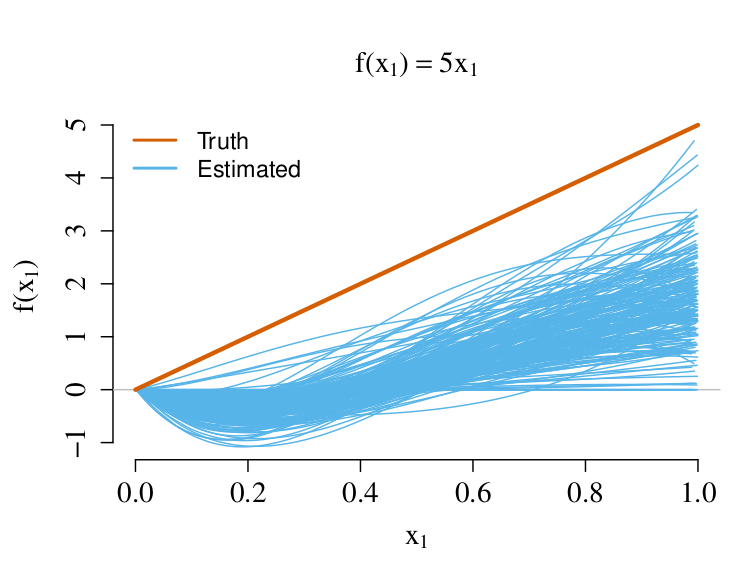
\includegraphics[width=0.5\linewidth]{figure/2021-10-12_10-18_1.png}}
	\subfloat{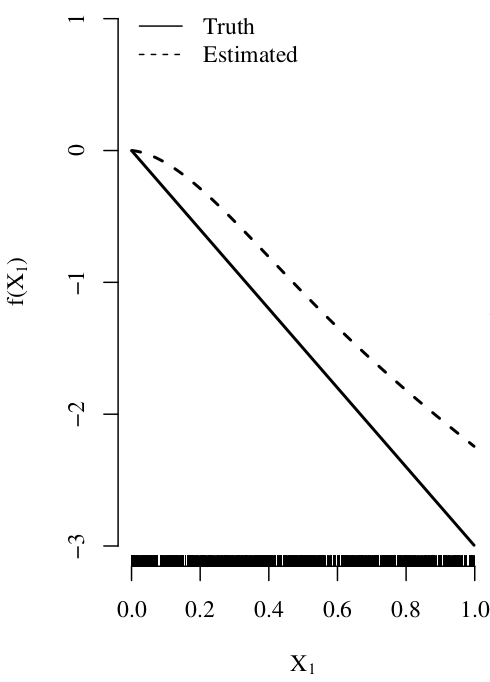
\includegraphics[width=0.5\linewidth]{figure/2021-10-12_10-18.png}}
	\caption{\textbf{Left}: True and estimated main effects across 200 replications for strong heredity \texttt{sail} in simulation scenario 1a). \textbf{Right}: True and estimated main effects for toy example given in section 1.3 of the main text.}
	\label{fig:X3}
\end{figure}
\end{reply}


%%%%%%%%%%%%%%%%%%%%%%%%%%%%%%%%%%%%%%%%%%%%%%%%%%%%%%%%%%%%%%%%%%%%%%%%%%%%%%%%%%%%%%%%%%%%%%%%%%%
%%%%%%%%%%%%%%%%%%%%%%%%%%%%%%%%%%%%%%%%%%%%%%%%%%%%%%%%%%%%%%%%%%%%%%%%%%%%%%%%%%%%%%%%%%%%%%%%%%%
%%%%%%%%%%%%%%%%%%%%%%%%%%%%%%%%%%%%%%%%%%%%%%%%%%%%%%%%%%%%%%%%%%%%%%%%%%%%%%%%%%%%%%%%%%%%%%%%%%%%%%%
%%%%%%%%%%%%%%%%%%%%%%%%%%%%%%%%%%%%%%%%%%%%%%%%%%%%%%%%%%%%%%%%%%%%%%%%%%%%%%%%%%%%%%%%%%%%%%%%%%%
%%%%%%%%%%%%%%%%%%%%%%%%%%%%%%%%%%%%%%%%%%%%%%%%%%%%%%%%%%%%%%%%%%%%%%%%%%%%%%%%%%%%%%%%%%%%%%%%%%%
%%%%%%%%%%%%%%%%%%%%%%%%%%%%%%%%%%%%%%%%%%%%%%%%%%%%%%%%%%%%%%%%%%%%%%%%%%%%%%%%%%%%%%%%%%%%%%%%%%%%%%%
%%%%%%%%%%%%%%%%%%%%%%%%%%%%%%%%%%%%%%%%%%%%%%%%%%%%%%%%%%%%%%%%%%%%%%%%%%%%%%%%%%%%%%%%%%%%%%%%%%%
%%%%%%%%%%%%%%%%%%%%%%%%%%%%%%%%%%%%%%%%%%%%%%%%%%%%%%%%%%%%%%%%%%%%%%%%%%%%%%%%%%%%%%%%%%%%%%%%%%%
%%%%%%%%%%%%%%%%%%%%%%%%%%%%%%%%%%%%%%%%%%%%%%%%%%%%%%%%%%%%%%%%%%%%%%%%%%%%%%%%%%%%%%%%%%%%%%%%%%%%%%%


\begin{point}
In the result("(2) Non-linearity simulation scenario"), the performance of the proposed method is not good(not stable) compared to others. It is necessary to check the estimation of intercept.
\end{point}


\begin{reply}
As mentioned in our response to point 2.7, we have revised the estimation of the intercept.  The performance of our proposed method in the ``(2) Non-linearity simulation scenario'' has now improved significantly, as shown in Figure~\ref{fig:scen2}. 
\begin{figure}[H]
    \centering
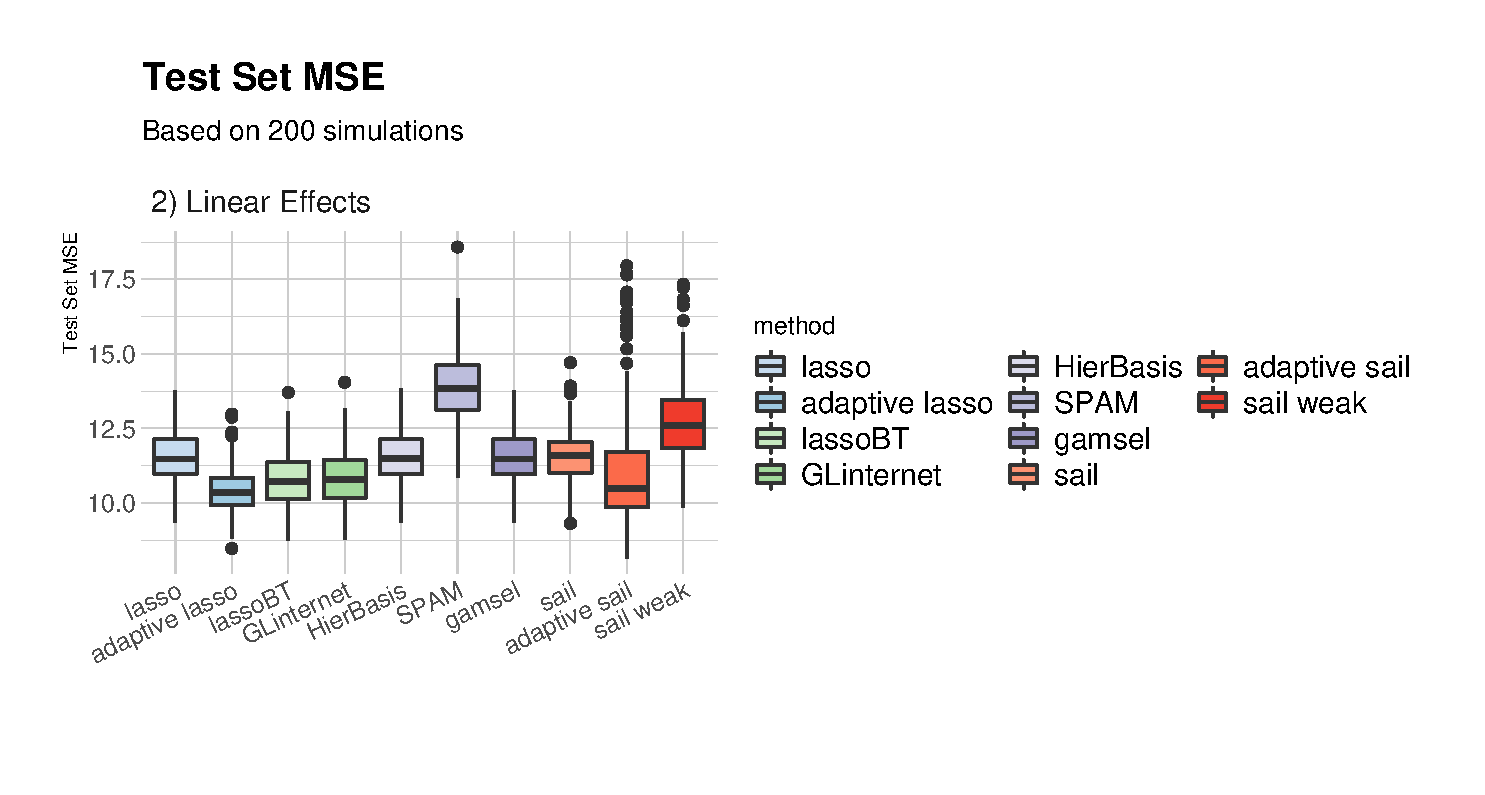
\includegraphics[width=\textwidth]{figure/mse_scen2_only.pdf}
    \caption{Simulation results across 200 replications for the (2) Non-linearity simulation scenario.}
    \label{fig:scen2}
\end{figure}

\end{reply}

\FloatBarrier

%%%%%%%%%%%%%%%%%%%%%%%%%%%%%%%%%%%%%%%%%%%%%%%%%%%%%%%%%%%%%%%%%%%%%%%%%%%%%%%%%%%%%%%%%%%%%%%%%%%
%%%%%%%%%%%%%%%%%%%%%%%%%%%%%%%%%%%%%%%%%%%%%%%%%%%%%%%%%%%%%%%%%%%%%%%%%%%%%%%%%%%%%%%%%%%%%%%%%%%
%%%%%%%%%%%%%%%%%%%%%%%%%%%%%%%%%%%%%%%%%%%%%%%%%%%%%%%%%%%%%%%%%%%%%%%%%%%%%%%%%%%%%%%%%%%%%%%%%%%%%%%
%%%%%%%%%%%%%%%%%%%%%%%%%%%%%%%%%%%%%%%%%%%%%%%%%%%%%%%%%%%%%%%%%%%%%%%%%%%%%%%%%%%%%%%%%%%%%%%%%%%
%%%%%%%%%%%%%%%%%%%%%%%%%%%%%%%%%%%%%%%%%%%%%%%%%%%%%%%%%%%%%%%%%%%%%%%%%%%%%%%%%%%%%%%%%%%%%%%%%%%
%%%%%%%%%%%%%%%%%%%%%%%%%%%%%%%%%%%%%%%%%%%%%%%%%%%%%%%%%%%%%%%%%%%%%%%%%%%%%%%%%%%%%%%%%%%%%%%%%%%%%%%
%%%%%%%%%%%%%%%%%%%%%%%%%%%%%%%%%%%%%%%%%%%%%%%%%%%%%%%%%%%%%%%%%%%%%%%%%%%%%%%%%%%%%%%%%%%%%%%%%%%
%%%%%%%%%%%%%%%%%%%%%%%%%%%%%%%%%%%%%%%%%%%%%%%%%%%%%%%%%%%%%%%%%%%%%%%%%%%%%%%%%%%%%%%%%%%%%%%%%%%
%%%%%%%%%%%%%%%%%%%%%%%%%%%%%%%%%%%%%%%%%%%%%%%%%%%%%%%%%%%%%%%%%%%%%%%%%%%%%%%%%%%%%%%%%%%%%%%%%%%%%%%


\begin{point}
Overall, many typos are very confusing to understand the proposed method in the current manuscript. Mainly, it is hard to follow the equations in the appendix. There are also many typos and inconsistent notations. For example, in equation (1) of the appendix, what is $\lambda_m^\theta$?
\end{point}


\begin{reply}
Thank you for raising this issue. $\lambda_m^\theta$ is a typo and should be $\lambda_m$. We have fixed this in the proofs given in Supplemental Section A. We have also re-checked the proofs and notation to ensure that it is indeed correct. The original notation in our proof was in fact more complicated and confusing. We tried to simplify the notation as much as possible. We summarize the original notation and the corresponding simplified notation in Table~\ref{tab:proofs}. We have also added this Table to the Supplemental Section A. 
	\begin{table}[H]
	    \centering
	    \begin{tabular}{|c|c|c|c|c|c|c|c|c|}
	    \hline
	       $\beta_{E}^{*}$ & $\btheta_{1}^{*\top}$ & $\btheta_{2}^{*\top}$ & $\ldots$ & $\btheta_{p}^{*\top}$ & $\gamma_{1E}^{*}$ & $\gamma_{2E}^{*}$ & $\ldots$ & $\gamma_{pE}^{*}$ \\
	       \rule{0pt}{4ex}    
	       $\boldsymbol{\phi}_{1}^{*\top}$ & $\boldsymbol{\phi}_{2}^{*\top}$ & $\boldsymbol{\phi}_{3}^{*\top}$ & $\ldots$ & $\boldsymbol{\phi}_{p+1}^{*\top}$ & $\boldsymbol{\phi}_{p+2}^{*\top}$ &
	       $\boldsymbol{\phi}_{p+3}^{*\top}$ & $\ldots$ & $\boldsymbol{\phi}_{2p+1}^{*\top}$ \\
	       \midrule
	       	       \rule{0pt}{4ex}    
$\lambda(1-\alpha)w_{E}$ & $\lambda(1-\alpha)w_{2}$ & $\lambda(1-\alpha)w_{3}$ & $\ldots$ &  $\lambda(1-\alpha)w_{p+1}$ & $\lambda\alpha w_{p+2,E}$ & $\lambda\alpha w_{p+3,E}$ & $\ldots$ &  $\lambda\alpha w_{2p+1,E}$\\
	       	       \rule{0pt}{4ex}    
$\lambda_1$ & $\lambda_2$ & $\lambda_3$ & $\ldots$ & $\lambda_{p+1}$ & $\lambda_{p+2}$ & $\lambda_{p+3}$ & $\ldots$ & $\lambda_{2p+1}$ \\
	       \hline
	    \end{tabular}
	    \caption{Correspondence between parameters used to simplify the notation in the proofs. The first row shows the actual parameters used in the loss function. The second row shows the corresponding parameters in the simplified notation. The third row shows the actual tuning parameters used in the penalty function. The fourth row shows the corresponding tuning parameters in the simplified notation. This correspondence greatly simplifies the notation used in the proofs. }
	    \label{tab:proofs}
	\end{table}


This notation then allows us to write down the \texttt{sail} estimates as
	\begin{equation}
	\widehat{\boldsymbol{\Phi}}_{n}=\argmin_{\boldsymbol{\Phi}}Q_{n}(\boldsymbol{\Phi})=-L_{n}(\boldsymbol{\Phi})+n\lambda_{m}\sum_{m=1}^{2p+1}\left\Vert \boldsymbol{\phi}_{m}\right\Vert _{2},
	\end{equation}

\end{reply}

\FloatBarrier

\bibliographystyle{apalike}
% Loading bibliography database
\bibliography{sail-refs}

\end{document}